In order to quickly iterate, work in parallel, and also work independently from the racecar on the project a simulation was implemented using Gazebo Fortress as a simulator.
Gazebo is a lightweight simulator which implements the SDF file format to describe robots and worlds and has close integrations with ROS2.
Since the project is constrained to using ROS2 Humble, the Fortress version was chosen since it is the recommended platform for Humble and Ubuntu jammy.
For the LiDAR sensor the Gazebo implementation is used and parametrized to fit the properties of the Sick LiDAR used by the F1Tenth hardware.
The RGB- and depth camera is modeled using the realsense camera sensor plugin available for gazebo \cite{realsense-gazebo}.

\subsection{Gazebo Communication}

Even though Gazebo Fortress is still under long-term-support (LTS) it does not come with python bindings for the Gazebo transport layer. 
This layer would usually handle all communication with the simulation using sockets and is available in newer version of Gazebo (like Ionic). 
However Gazebo Fortress exposes services over a CLI. This can be used to implement the Gazebo message-protocol using system calls which can then be executed using python. 
The whole implementation is available in the Github repository of this project and implements the different message types using the pydantic framework. 
The messages are then serialized into strings and sent to Gazebo over a system call. 
Even though some service calls can be batched for example when spawning many entities (cones) at once, 
this approach introduces some delays and the system calls can also timeout when send with a high frequency.\\
\newline
The main services made available this way are:

\begin{itemize}
\item "/world/:world:/create"
\item "/world/:world:/create\_multiple"
\item "/world/:world:/set\_pose"
\item "/world/:world:/remove"
\item "/world/:world:/control"
\end{itemize}


The \textbf{create} service can be used to instantiate SDF-files into a running Gazebo simulation where the models are instantiated as a blocking call (appear immediately from the perspective of the simulation). \textbf{create\_multiple} can be used to batch many calls to the create service to reduce the load. \textbf{set\_pose} is a service for manipulating the position and rotation of entities in the simulation. In this project it is used to set the position and rotation of the vehicle to a neutral position after a reset call to the environment.\\
The \textbf{remove} service can be used to remove entities from the simulation. This call can unfortunately not be batched resulting in very long execution times when trying to remove many entities from the simulation. At first this was supposed to generate a new track every time the environment was reset but the associated rebuild time resulted in infeasible training times (over a minute for a rebuild).\\
\textbf{control} is a service able to start or stop the simulation or run it for a certain amount of time steps. This was first used to make the `step` function of the environment deterministic but resulted in too many system calls for Gazebo which resulted in data inconsistencies and dropped calls.

\subsection{Track Generation}

Since the Formula Student tracks are defined by cones we implemented a generator for tracks with some free parameters like size, width, cone distance and shape.
The track generation algorithm samples $n$-points from a normal distribution $\mathcal{N}(\mu, \sigma^2)$ with $\mu = 0$ and $\sigma = 1$ to create a 2D point cloud. These points are then used to calculate the concave hull to retrieve the outer shape of the point cloud. At first I tried using the convex-hull of the point cloud but a concave-hull does not contain left-curves (when traversed clock-wise) which would truncate the action space by half since only positive steering angles would be required to traverse the track. This would lead to poor generalization when tested in the real world where tracks will contain left curves. The set of points of the concave hull is then z-normalized (subtraction of mean divided by the standard deviation) and then scaled to the desired track size.
Afterwards a polygon is created from the concave hull and buffered by the track width $w$ to produce an inner and outer polygon boundary defining the border of the track. The track can now still contain some sharp curves that are not fit for the car platform since it can not steer around them. To solve this, Chaikins corner cutting algorithm \cite{chaikin1974algorithm} was applied to the borders where the number of refinements $r$ is a free parameter.\\
\newline
The application of the corner cutting algorithm now leaves the borders of the track with sparse data points on straight sections and dense data points on the refined sections where sharp curves occurred. To end up with an even distribution of cone positions the borders are resampled using linear interpolation.
In order to introduce some more complex track environments, the $d$ parameter can be used to pull $d$ evenly spaced points from the concave hull inwards, leading to sharper curves.

\begin{algorithm}[tb]
\caption{Track Gen}
\label{alg:track-gen}
\begin{algorithmic}
\State {\bfseries Input:} $n$, $s_x$, $s_y$, $w$, $r$, $\alpha$, $d$
\State $X_n \sim \mathcal{N}(\mu,\,\sigma^{2})$
\State $C_0$ = alphaShape($X, \alpha$)
\State $C_0$ = applyDents($C_0, d$)
\State $C_\text{norm}$ = zNorm($C_0$)
\State C = stack($C_x \cdot s_x, C_y \cdot s_y$)
\State $T_\text{outer}$ = buffer($C_\text{norm}, w/2$)
\State $T_\text{inner}$ = buffer($C_\text{norm}, -w/2$)
\State $T_\text{router}$ = chaikin($T_\text{outer}, r$)
\State $T_\text{rinner}$ = chaikin($T_\text{inner}, r$)
\State $T_\text{souter}$ = resample($T_\text{router}$)
\State $T_\text{sinner}$ = resample($T_\text{rinnter}$)
\State {\bfseries Return:} $T_\text{souter}, T_\text{sinner}$
\end{algorithmic}
\end{algorithm}

Figure \ref{fig:track} shows the generated track for the environment from a top-down perspective. The blue dots describe the cone positions. The origin of the track is in the middle at the very top since the coordinate system in Gazebo uses the y-direction as a forward direction. The track is then traversed in clock-wise direction.

\begin{figure}[ht]
\vskip 0.2in
\begin{center}
\centerline{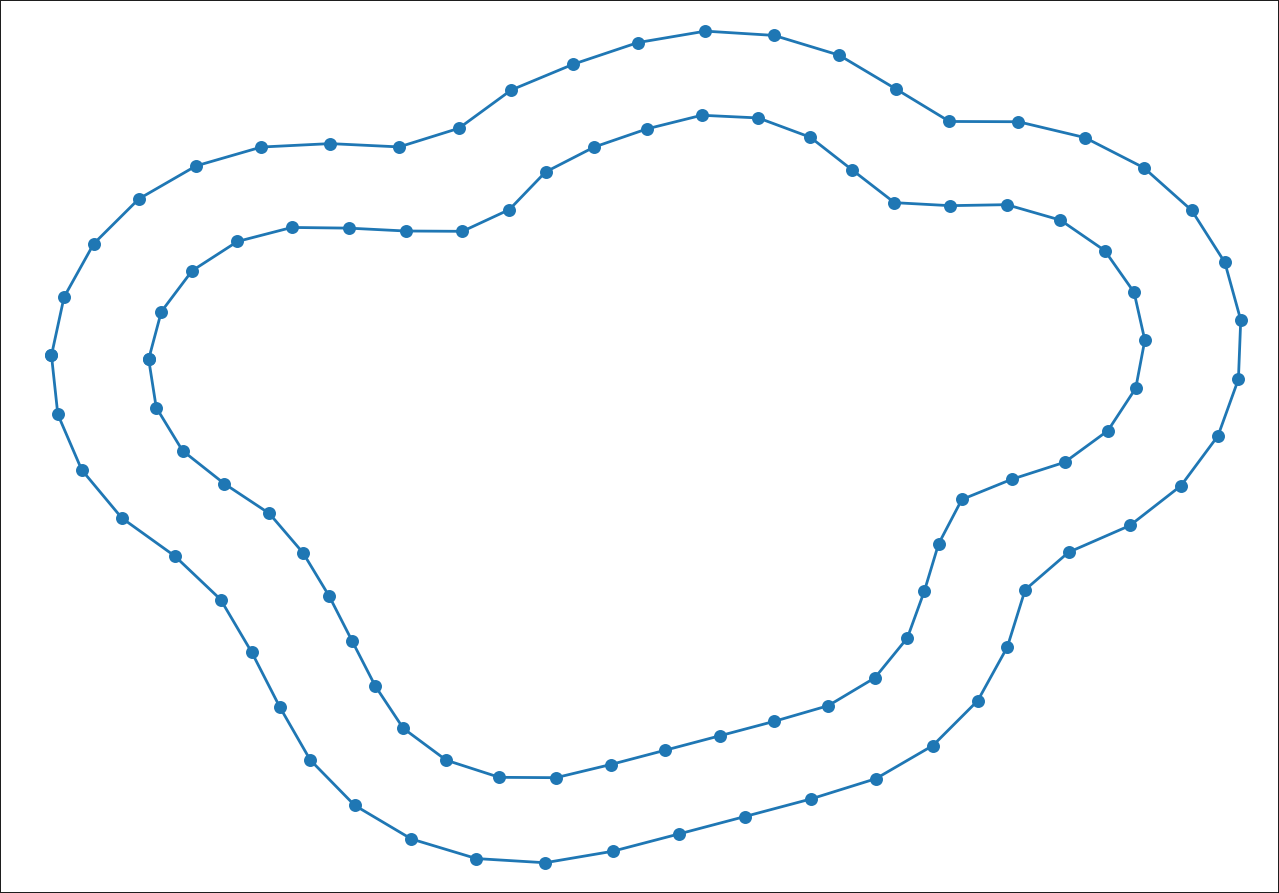
\includegraphics[width=\columnwidth]{track.png}}
\caption{The generated track boundaries using the RNG seed 42. Blue dots mark the positions of cones.}
\label{fig:track}
\end{center}
\vskip -0.2in
\end{figure}

\subsection{Gazebo ROS2 Communication}

Apart from system calls to interact with services provided by Gazebo Fortress we use the ROS-Gazebo-Bridge to convert the topics and data types published in Gazebo to ROS2. 
This is a transport layer that is available in python and can be launched using ROS2 and the regular python launch file syntax. 
This conversion process is very resource intensive which is why only the LiDAR sensor and the odometry can be updated with a high frequency.

